\documentclass{article}

\usepackage{arxiv}

\usepackage{lipsum}

\usepackage[utf8]{inputenc} % allow utf-8 input
\usepackage[T1]{fontenc}    % use 8-bit T1 fonts
\usepackage{hyperref}       % hyperlinks
\usepackage{url}            % simple URL typesetting
\usepackage{booktabs}       % professional-quality tables
\usepackage{amsfonts}       % blackboard math symbols
\usepackage{nicefrac}       % compact symbols for 1/2, etc.
\usepackage{microtype}      % microtypography
\usepackage{graphicx}

\graphicspath{ {../} }

\usepackage{natbib}
\usepackage{amsmath}
\usepackage{amssymb}
\usepackage{amsthm}
\usepackage{stmaryrd}
\usepackage{algorithmic,algorithm}
\usepackage{graphicx}
\usepackage{caption}
\usepackage{subcaption}
\usepackage{tikz}
\usetikzlibrary{positioning}
\usepackage{comment}


\newcommand{\cX}{\mathcal{X}}
\newcommand{\cL}{\mathcal{L}}
\newcommand{\cY}{\mathcal{Y}}

\newcommand{\bX}{\mathbf{X}}
\newcommand{\bY}{\mathbf{Y}}

\newtheorem{definition}{Definition}
\newtheorem{remark}{Remark}
\newtheorem{proposition}{Proposition}
\newtheorem{corollary}{Corollary}

\title{Coordination of Connected Vehicles using Reinforcement Learning}

\author{
 Jeroen van Riel \\
Eindhoven University of Technology\\
  \texttt{j.a.a.v.riel@student.tue.nl} \\
}

\begin{document}
\maketitle


\section{Motivation}

Given the growing number of connected vehicles (CVs), an interesting question
becomes how traffic can be handled efficiently in scenarios where every vehicle
can be fully controlled by a single traffic manager with full information and
perfect communication. Studying this question is important because it provides
an upper bound on how efficiently traffic could be handled in such a scenario by
neglecting issues related to communication latency, partial information, and
decentralized control.

The problem we would like to consider is in essence about finding trajectories
of vehicles through a network of intersections while optimizing for some measure
of (economic or social) efficiency, to which we will refer as \textit{trajectory
  planning}. Even when the route of a vehicle is fixed, there is still a lot of
freedom in determining the speed profile over the course of this route. Previous
studies have considered methods that are based on a two-stage decomposition:
first determine the times when a vehicle crosses each intersection along its
route, then compute the speed profile based on these times.

% movement planning is difficult

In general, efficiently planning the movement of vehicles through a road network is
a difficult problem because control of one intersection directly influences the
arrival process of vehicles of nearby intersections. In dense urban networks,
these interactions become highly complex, which makes modeling the dynamics from
first principles very difficult. Furthermore, the inherent nonstationarity of
traffic demand, with fluctuations throughout the day, makes it difficult to
design controllers that adapt their policy to these changes.

Deep learning methods have been proven to be very useful in capturing highly
complex relationships that are otherwise very hard to capture from first
principles. Furthermore, deep reinforcement learning methods have been
successfully applied to automatically select good policies from very
high-dimensional classes of policies, parameterized through deep neural
networks. The aim of this proposal is to explore how deep reinforcement learning
could be employed to develop procedures for trajectory planning of CVs in
existing urban networks of intersections.


%%------------------------------------------------------------------------------
\section{Literature Analysis} \label{sec:broadliterature}

% introduce section

This section highlights some of the literature on traffic control by discussing
illustrative classical methods for signalized intersections and giving an
overview of recent applications of reinforcement learning techniques. The second
part discusses relevant work on idealized traffic models featuring only
connected autonomous vehicles (CVs).

\subsection{Signalized Intersections}

% traffic prediction and control -> signalized intersection

A vast amount of literature is available on methods for predicting and
controlling road traffic. In particular, the context of networks of signalized
intersections has received a substantial amount of attention. In most of these
works, the main goal is to derive policies for setting traffic light signals
such that traffic is handled as efficiently as possible, which is commonly
measured in terms of the total delay experienced by all vehicles over some
period of time. It has often been recognized that efficient control schemes
should include some degree of coordination among the signal controllers at
individual intersections, which is commonly refered to as \textit{coordination}.
A well-known example of such a strategy is given by so-called \textit{green
  waves} on arterial roads.

% MILP methods

Early methods such as MAXBAND \cite{mcshane_traffic_1990} aimed to synchronize
multiple neighboring intersections, by tuning the timing offset between cyclic
signal plans of the intersection, in order to achieve coordination. An
interesting derivative of the original MAXBAND formulation is the PAMSCOD system
\cite{he_pamscod_2012}, which is a framework that consists of a model for
identifying platoons and a Mixed-Integer Linear Program (MILP) formulation for
scheduling these platoons throughout a network in an online fashion. Under the
assumption that the traffic controller receives actual position and speed
information from a certain percentage of vehicles, a heuristic algorithm is
proposed to identify platoons and estimate their size and expected arrival time
at downstream intersections. The order in which these platoons cross the
intersections in the network is then optimized using a MILP formulation that
minimizes a combination of delay experienced at the next two encountered
intersections. A solution provides the green times of signals for a fixed number
of cycles in the future, so their method is a form of \textit{rolling horizon
  optimization}.

% microsimulator

Because deploying control policies in existing road infrastructure is often
non-trivial, evaluation is often done by using a so-called \textit{traffic
microsimulator} like SUMO \cite{lopez_microscopic_2018} or VISSIM. In contrast to
\textit{macroscopic models}, which aim to capture traffic dynamics in terms of
aggregated quantities for large numbers of vehicles, such simulators try to
capture the behavior of individual vehicles very precisely, such that realistic
behavior on a larger scale emmerges automatically.

% reinforcement learning

Recently, there has been a growing interest in using reinforcement
learning algorithms for developing efficient traffic signal control policies
\cite{noaeen_reinforcement_2022}. Most of this work is centered around a microsimulator to which an off-the-shelf reinforcement learning algorithm is applied in combination with
some kind of neural function approximation to encode the high-dimensional state
space.
%
The obtained results are often very impressive in terms of pure performance,
while relying on the availability of lots of computational power. Unfortunately,
due to the model-free nature of the learning methods used, these studies do not
provide much insight into the learned policies that could be exploited to
derive methods that are computationally more efficient.
%
Furthermore, the challenge of automatically learning how to achieve coordination
among multiple intersections without any prior knowledge has been identified as
one of the key remaining issues in this line of research.


\subsection{Connected Vehicles}

% full control of vehicles -> trajectory generation

Assuming that that all vehicles in the network are fully connected poses a lot
of interesting new research questions \cite{gholamhosseinian_comprehensive_nodate}. However, the main problem
of allocating intersection access time to vehicles remains a central issue. In
this context, classical methods like MILP solving \cite{fayazi_mixed-integer_2018} are still an
important tool for solving such \textit{temporal} optimization problems.
However, the current setting allows us to consider optimization in the
\textit{spatio-temporal} domain. With signalized intersections and human
drivers, trajectories of individual vehicles cannot be directly controlled, but
under the current assumption \textit{trajectory planning} becomes relevant.
This issue has already been
studied for the \textit{conflict zone} of intersections. For example, in
\cite{li_temporal-spatial_2019-1} the trajectories of vehicles are modeled as volumes in time and space
that can be used to characterize conflicting trajectories.

% single intersection

For a single intersection, the two-stage approach in \cite{feng_spatiotemporal_2018} first computes
access times using dynamic programming and use these to compute conflict-free
trajectories as solutions to an optimal control problem. A similar approach was
taken in \cite{timmerman_platoon_2021}, where intersection access times are determined by
simple policies from queueing theory instead. The performance of their method
was analyzed using results from \textit{polling theory}.

% temporal domain -> scheduling

When the optimization objective only considers delay at the intersection, i.e.,
only in the temporal domain, the problem of finding efficient access times can
be interpreted as a variant of \textit{single machine scheduling}. More
precisely, using terminology from the \textit{machine scheduling} literature
\cite{pinedo_scheduling_2016}, it can be shown that the problem reduces to a
single machine scheduling problem with release dates, job families with chain
precedence constraints (corresponding to lanes), family-dependent setup times
and total completion time objective.

% online scheduling

Machine scheduling is a widely studied subfield of combinatorial optimization
with a wide range of applications in, for example, manufacturing and healthcare.
Dealing with situations in which not all information about jobs is available
upfront is known as \textit{online scheduling} \cite{guerreiro_online_2023, vestjens_-line_1997}. The
performance of an online scheduling policy depends highly on how information is
disclosed, so different metrics are necessary for evaluation. A common approach
is to consider the worst-case performance  compared an optimal \textit{offline
algorithm} that has access to all future information. Alternatively, an explicit
specification of the information disclosure process may be assumed to analyze
performance in expectation. This kind of analysis is particularly important for
our current context of road traffic control, because demand for mobility is
highly unpredictable.


%%------------------------------------------------------------------------------
\section{Problem Formulation and Objective}

This section provides a sketch of our model of coordination of connected
vehicles through a network of intersections which will serve as the main
conceptual model throughout the project. Vehicles are represented as little dots
and arrive to a graph over time. They follow a fixed deterministics route
towards a final node, where the vehicle leaves the system. The goal of the
traffic controller is to determine how vehicles move exactly along their route
by providing their speed profiles, while satisfying some constraints on the
interaction between vehicles in lanes and at intersections that are due to
safety considerations.

% vehicle driving through network and traffic controller
Let $G$ be some road network, modeled as a directed graph, with intersections
represented by nodes and lanes represented by arcs. We assume that vehicle are
not allowed to overtake, so they need to stay in their lane.
%
We assume that routes are fixed and deterministic.
%
For each vehicle $j$, let its route be denoted by $R_{j}$, which is encoded as a
sequence of nodes. Vehicle $j$ enters the network at some external node
$R_{j}(0)$ at time $r_{j}$ and then visits the $n_{j}$ intersections
$R_{j}(1), \dots, R_{j}(n_{j})$ until it reaches the exitpoint
$R_{j}(n_{j} + 1)$, where it leaves the network.
% define common path
 See Figure~\ref{fig:intersection-graph-example} for an
illustration.

\begin{figure}[t]
  \centering
  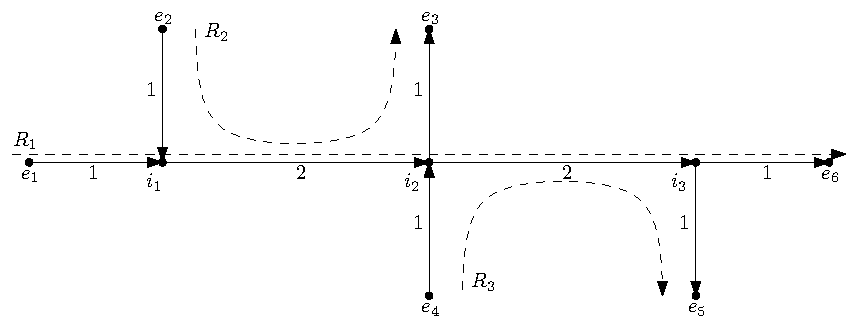
\includegraphics[width=1.0\textwidth]{figures/intersection-graph-example.pdf}
  \caption{Example graph $G$ with three intersection $i_{1}, i_{2}, i_{3}$ and three
    vehicles routes, indicated by $R_{1}, R_{2}$ and $R_{3}$.
    The external nodes are labeled as $e_{1}, \dots, e_{6}$. The weight
    (travel time) of each arc is indicated next to it.}
  \label{fig:intersection-graph-example}
\end{figure}


We assume that there is one \textit{central traffic controller} that knows the
exact position of every vehicle in the network. Let $x_{j}(t)$ denote the
position of vehicle $j$ on its route $R_{j}$ at time $t \geq r_{j}$. We also use
the notation $x_{ij}(t)$ to denote the position in the lane on the route of $j$
leading to the $i$th intersection on its route, see
Figure~\ref{fig:general-model}. Furthermore, let $v_{j}(t)$ and $a_{j}(t)$
denote the speed and acceleration, respectively, of vehicle $j$ at time $t$.

\begin{figure}[b]
  \centering
  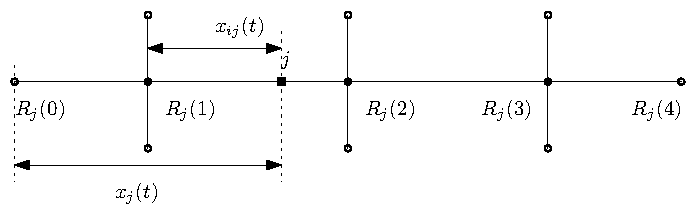
\includegraphics[width=0.9\textwidth]{figures/general_traffic_model.pdf}
  \caption{Illustration of a network of intersections with the position of some
    vehicle $j$ given in two ways.}
  \label{fig:general-model}
\end{figure}

% trajectory constraints: smoothness, velocity and acceleration
The traffic controller determines trajectories $x_{j}(t)$
satisfying some kind of smoothness and safety constraints. For example, we may
impose maximum/minimum speed and acceleration constraints
\begin{align}
    v_\text{min} & \leq v_j(t) \leq v_\text{max} , \\
    a_\text{min} & \leq a_j(t) \leq a_\text{max} .
\end{align}


% lane switching: merge point (head of common path)
Given a node $i$, let $t_{ij} = t_{ij}(x_{j})$ denote the time when vehicle $j$
crosses $i$. Between crossing of vehicles from different lanes, we enforce a
\textit{safe lane-switching} time $s_{\text{lane}}$. Whenever a pair of distinct
vehicles $j \neq l$ crosses the same intersection $i$, we require that either
\begin{align}
  t_{ij} + s_{\text{lane}} \leq t_{il} \quad \text{ or } \quad t_{il} + s_{\text{lane}} \leq t_{ij} .
\end{align}
% following distance and overtaking: tail of common path
Furthermore, when two vehicles $j$ and $l$ are driving in the same lane we
require some minimum \textit{safe following distance} $d_{\text{follow}}$. For
all pairs of distinct vehicles $j \neq l$, we require that
\begin{align}
  \label{eq:following-distance-constraint}
  x_{ij}(t) + d_{\text{follow}} \leq x_{il}(t) \quad \text{ or } \quad x_{il}(t) + d_{\text{follow}} \leq x_{ij}(t) ,
\end{align}
at all times $t$ when both vehicles are driving towards a common intersection $i$.

The objective for the traffic controller is to compute trajectories while
minimizing some performance measure, e.g., the total delay experienced by
vehicles at intersections, which is equivalent to minimizing
\begin{align}
  \label{eq:obj}
  \sum_{j} \sum_{i \in R_{j}} t_{ij} ,
\end{align}
where the sum is taken over all indices of vehicles that were present in the
network during a certain time interval.

\subsection{Objective}

In general, our goal is to develop computationally efficient methods for solving
the problem sketched above. More specifically, we aim to employ existing
off-the-shelf reinforcement learning techniques to learn policies for efficient
trajectory planning.

A proven approach is to decompose the solution into a part that schedules the
intersection access times and a part that uses this schedule to compute
continuous conflict-free trajectories. Inspired by the idea of integrating
machine learning methods with combinatorial optimization
\cite{bengio_machine_2020}, we aim to study an alternative method of scheduling
access times based on a graph representation that allows us to apply
reinforcement learning \cite{zhang_learning_2020}.

Besides exploiting this explicit two-stage decomposition, we would like to
consider a spatio-temporal scheduling model to generate trajectories in a more
direct way. We have a preliminary solution in this direction that we would like
to validate. Ideally, we would also like to learn policies for this model using
reinforcement learning.


%%------------------------------------------------------------------------------
\section{Research Approach} \label{sec:approach}

This section provides an overview of our current concrete research ideas.
Because temporal scheduling is still not fully understood in even very simple
cases, we will at first ignore the spatial issues by focusing on methods of
intersection access scheduling for single intersections and networks of
intersections. After that, we propose a model for developing trajectory planning
algorithms that do not rely on a two-stage scheduling decomposition.

%%------------------------------------------------------------------------------

\subsection{Single Isolated Intersection}
\label{sec:single}

Before investigating coordination across multiple intersections, we first
revisit the special case with a single isolated intersection. This already
offers many interesting questions that may help us later in distinguishing which
problems arise due to network effects or spatial constraints.

% MILP

The single intersection scheduling problem can thought of as a variant of a
single machine scheduling problem, in which jobs needs to be assigned time on a
single machine. Like other single machine problems, the current problem can be
rather naturally formulated as a Mixed-Integer Linear Program (MILP) by introducing
binary decision variables for the ordering of vehicles from different lanes.
Relying on the current power of MILP solvers, e.g. Gurobi \cite{gurobi}, this
provides an exact solution to the problem, assuming that all arrivals are known
from the start.

% rl

In order to apply reinforcement learning, we need to precisely specify the
sequential decision making process as a Markov Decision Process (MDP). We propose
to study a simple \textit{dispatching} policy that computes a schedule by
simulating the behavior of a traditional traffic light. More precisely, the
policy decides which vehicle is allowed to cross the intersection next in the
following way. The agent takes a vector of the next $h$ earliest crossing times
for both lanes as input and decides whether to keep serving the current lane or
to switch to the other lane. The number $h$ of next crossing times the
controller sees is referred to as the \textit{horizon}. In a sense, this
resembles the way traffic lights switch between \textit{phases} at most existing
signalized intersection.

% reinforcement learning algorithm

Choosing the most efficient reinforcement learning algorithm for our current
model is not our main concern. Therefore, we will settle with an off-the-shelf
implementation of deep Q-learning with experience replay
\cite{mnih_human-level_2015} for this single intersection environment. Once a
policy has been trained that performs reasonably well in terms of the
optimization objective, we can analyze it in the following ways:

\begin{itemize}

  \item \textbf{Comparison.} First of all, we can compute optimal solutions for
        small instances, so the approximation ratio can be computed precisely in
        these cases by comparing the objective value to the optimal found by a
        MILP solver. Furthermore, the performance can be compared to existing
        policies under the assumption of a fixed distribution of the arrivals
        $r_j$. Examples of policies to compare with are exhaustive service, in
        which the current lane is served as long as vehicles are waiting there,
        or the gated policy from \cite{timmerman_platoon_2021}.

  \item \textbf{Effect of horizon size.} It is possible to experiment with
        different sizes of the horizon. For a fixed distribution of the arrivals
        $r_j$, we expect that the performance of the learned policy does not
        improve significantly beyond a certain horizon size.

  \item \textbf{Generalization.} A central question in reinforcement learning is
        the issue of generalization. For example, we could assess how well the
        trained policy performs with a (slightly) different distribution of
        $r_j$. Furthermore, when considering more than two incoming lanes, an
        interesting question is whether we can train policies that generalize
        across different numbers of lanes.

  \item \textbf{Policy interpretation.} For learned policies that perform really
        well, it might be worthwhile to analyze their behavior a bit further in
        the hope of discovering structure that can be used to define better
        policy spaces. Two possible ways of doing this are by providing certain
        ``test states'' to see which actions get selected and providing test
        instances for which we know the optimal solution to see how close the
        schedule produced by the policy is.

\end{itemize}


\subsection{Network of Intersections}

The next step is to consider networks of connected intersections. Before
considering the problem in the spatial and temporal domain in a unified fashion,
we treat the scheduling problem for multiple intersections. More precisely, we
again assume there is no limit on the number of vehicles that can be present in
lanes between intersection. This provides a lot of new interesting questions,
because decisions taken at an intersection influence the arrival process of
downstream intersections. Under these assumptions, we obtain a variant of the
well-known and widely studied job shop scheduling problem
\cite{pinedo_scheduling_2016}. Job shop problems are a particular type of
multi-machine scheduling problem in which jobs consist of consecutive stages,
where each stage must be executed on a different machine.

% solve as MILP

Again, the offline variant of this problem can be formulated as a MILP and
solved to optimality with readily available solvers. However, we expect that
this approach does not scale well in terms of the network size and number of
vehicles. Therefore, in order to solve problems at a real-world scale, we need
to focus on finding good heuristics. Our results for the single isolated
intersection can be readily applied to the current model by controlling each
intersection independently by the single intersection dispatching policy. While
this is still interesting to try, a different approach is required in order to
obtain coordination among intersections.

% based on disjunctive graph

Instances of job shop scheduling can be adequately represented as a graph that
encodes the precedence constraints between jobs. This graph is called the
\textit{disjunctive graph}, because a subset of the arcs encodes the disjunctive
ordering decisions between jobs on the same machine (vehicles approaching the
same intersection in the current context). A recent study
\cite{zhang_learning_2020} has exploited this structure to obtain a principled
approach to applying reinforcement learning to the job shop problem. Their
current method is only applicable as an offline scheduling algorithm, so we
would like to extend their method such that it can also be applied in an
online setting.

% discuss interesting questions
In addition to the questions discussed in the previous section, the current
network setting provides the following additional directions of inquiry.

\begin{itemize}

  \item \textbf{Coordination along arterial road.} A widely studied phenomeon in
        traffic signal control is coordination along a series of arterial
        intersections. The idea is that aligning the timing of traffic signal
        phases along a series of connected intersections that handle relatively
        large fraction of total traffic is often a good strategy to optimize
        overall delay in the network. Consider a network with a couple of
        intersections in series with some minor adjacent roads. By using an
        instance with a very regular arrival pattern on the main arterial and a
        limited arrival rate at the minor roads, we can assess coordination by
        measuring whether the policy actually exploits the regularity of the
        arrivals.

  \item \textbf{Platoon splitting.} For a single intersection, it has been shown
        that splitting platoons of vehicles is never beneficial
        \cite{limpens_online_2023}. However, for more than one intersection, it
        can be shown that this platoon preservation theorem no longer holds,
        even in some very simple situations. It would be interesting to
        understand better why this happens by characterizing this kind of
        situation.

  \item \textbf{Generalization across network topologies.} Ideally, the
        scheduling method can be used regardless of the the network
        topology at hand. In that case, it is possible to study how well a
        policy trained on some network topology generalizes to other topologies.
        This further motivates our idea of using the job shop disjunctive graph,
        which could help in making the policy topology-agnostic.
\end{itemize}


\subsection{Finite Buffers Model}

% location delays

In the models discussed above, we assumed that vehicles do not interact in
lanes, hence it is possible for an unbounded number of vehicles to wait in a
lane at any given time. However, in real-world traffic networks, the maximum
possible number of vehicles is limited by spatial constraints and even depends
non-trivally on the speeds of individual vehicles. Therefore, we propose a model
that incorporates this aspect by considering the position of vehicles in lanes.
Instead of encoding the precise location in a continuous sense, we divide each
lane in a finite number of locations. For a given vehicle, the controller has to
decide how long it should wait on each location. For large number of locations
per lane, this method allows us to approximate continuous trajectories through
interpolation.

% more precise

We illustrate our idea for a single intersection. Assume that it takes constant
time $\Delta t$ for a vehicle to travel to the next location. For each lane $k$,
let $m_{k}$ denote the number of locations, excluding the entrypoint. Let the
locations of lane $k$ be identified by increasing numbers
$\mathcal{L}(k) = (1, \dots , m_{k})$, where the last one corresponds to the
intersection. In the following variable definitions, we will not
explicitly mention the dependency on the lane to keep notation simple. Let
$y_{ij}$ denote the time at which vehicle $j$ departs from location
$i \in \{ 0, \dots, m_{k} \}$, then $y_{ij} + \Delta t$ is the arrival time of
vehicle $j$ at location $i+1$. To simplify notation, we define
$\bar{y}_{ij} = y_{i-1,j} + \Delta t$ to be the arrival time of vehicle $j$ at
location $i$. For every location $i$ and vehicle $j$, we require
\begin{align}
  \label{eq:constr1}
  \bar{y}_{ij} \leq y_{ij}
\end{align}
and the difference between these two quantities is called the \textit{location
  delay}. For each pair of consecutive vehicles in the same lane $k$ with
precedence constraint $j \rightarrow l$ (so vehicle $l$ arrived later than $j$),
we have the constraints
\begin{align}
  \label{eq:constr2}
  y_{ij} + p \leq \bar{y}_{il} ,
\end{align}
for every location $i$ in their lane.
%
Next, we model the safety constraints involving vehicles from
different lanes that cross a common intersection $i$. Let $j$ be some vehicle in lane
$k(j)$, then let let $y_{j}$ denote the departure time from the intersection, so
we have $y_{j} = y_{ij}$ with $i=m_{k(j)}$. Similarly, let $\bar{y}_{j}$ denote
the arrival time of $j$ at the intersection, so we have
$\bar{y}_{j} = y_{i-1,j} + \Delta t$ with $i = m_{k(j)}$. From
constraints~\eqref{eq:constr2}, we see that it makes sense to say that vehicle
$j$ \textit{occupies the intersection} during the interval
\begin{align}
  [\bar{y}_{j}, y_{j} + p] .
\end{align}
We require an additional \textit{switch-over time} $s$ whenever the next vehicle
to occupy the intersection comes from a different lane.
%
This results in the additional constraints
\begin{align}
  \label{eq:3}
  y_{j} + p + s \leq \bar{y}_{l} \quad \text{ or } \quad y_{l} + p + s \leq \bar{y}_{j} ,
\end{align}
for all pairs of conflicting vehicles $j \neq l$ that approach intersection $i$
from distinct lanes.


% network

Because of the discrete nature of the model, it is straightforward to formulate
it as a MILP, which allows us to obtain optimal schedules $y$ for objectives
similar to \eqref{eq:obj}. However, as the number of variables grows rapidly
with the values of $m_{k}$, we do not expect this approach to scale well.
Therefore, we would like to investigate how we could employ reinforcement
learning to solve this problem, similarly to how we do this for the job shop
variant for network scheduling.

A major question is how to structure the policy for determining location delays
for vehicles in a online setting. It might seem straightforward to let the
controller determine, for every vehicle, the location delays of the next couple
of locations. An alternative approach would be to have the controller set a
location delay for each location, independently of the vehicles. In a sense,
this is somewhat similar to the dispatching policy for the single intersection
scheduling problem, in that the problem is agnostic with respect to the number
of vehicles present in the network.

%%------------------------------------------------------------------------------
\section{Timeline}

This section provides a rough sketch of the timeline of the project from now on.
Counting from the week of February 5th onwards, I propose a rough division of
the project over approximately 22 weeks, aiming to finish by the end of July
2024.

At this point, we have already developed some methods for each of the three
models. We are currently analyzing the trained policies for the single
intersection case. After this, we try to extend the job shop scheduling method
with disjunctive graphs to online problems. The ordering of parts in the
following plan is based on the decomposition above. However, we are considering
working on the interpolation method for the finite buffers model when we are
finished with the analysis of the single intersection, because we want to have
an early proof of concept to check whether the proposed approach actually makes
sense.

\begin{itemize}

  \item \textbf{Single intersection environment (done).} Develop a Gymnasium
        \cite{towers_gymnasium_2023} environment for the single intersection
        dispatching policy.

  \item \textbf{DQN agent for single intersection (done).} Using the
        off-the-shelf DQN implementation provided by CleanRL
        \cite{huang2022cleanrl}, we managed to train good policies for some
        examples of arrival distributions.

  \item \textbf{Analyze performance of single intersection policy (started, 2
        weeks).} We are currently comparing the performance of the trained
        policies with optimal solutions found by solving the corresponding MILP
        for small instances. As we indicated in Section~\ref{sec:single}, we
        would also like to study the effect of the horizon size $h$ and some
        basic study of generalization over different arrival distributions.

  \item \textbf{Interpret single intersection policy (2 weeks).} We think that
        there is some particular structure to the optimal policies for the
        simple single intersection scheduling problem. Therefore, we would like
        to try understanding the behavior of the trained policies a bit better
        in the hope of discovering some simple rules that can be used to develop
        more efficient algorithms.

  \item \textbf{Adapt disjunctive graph-based scheduling (4 weeks).} The job
        shop scheduling method based on the disjunctive graph
        \cite{zhang_learning_2020} needs some slight adaptations in order to be
        applicable to the variant of job shop that is relevant for scheduling in
        networks. The authors provide reinforcement learning code and a Gym
        environment. However, their code is not very well documented, so we are
        considering a rewrite of the necessary parts.

  \item \textbf{Analyze network policies (1 week).} Once we are
        able to solve the job shop variant in an offline setting, we can do some
        preliminary experimentation and performance analysis.

  \item \textbf{Define how to adapt the disjunctive graph for online scheduling (2
        week).} We have a rough idea of how the disjunctive graph scheduling
        method could be extended to be applicable in an online fashion. The
        basic idea is to just extend the disjunctive graph every time new
        vehicles (jobs) arrive. Therefore, the main challenge is finding a
        suitable deep learning embedding of this graph that can deal with these
        kinds of extensions.

  \item \textbf{Implement online scheduling (3 weeks).} We expect that we need
        to reconsider the graph neural network that is used to learn an
        embedding of the disjunctive graph in order to get our intended method
        working.

  \item \textbf{Analyze online performance of network policies (2 weeks).} Like
        we did for the single intersection case, the learned policies should be
        analyzed in terms of performance. Furthermore, we should investigate
        whether the policies show some degree of coordination on intersections
        along arterial roads.

  \item \textbf{Define interpolation for finite buffers model (2 weeks).} Our
        current definition of the finite buffers model does not yet involve
        continuous trajectories. We still need to exactly define how the
        location delays can be used to compute non-overlapping vehicle
        trajectories.

  \item \textbf{Finite buffers model environment (started, 2 weeks).} Given the
        interpolation method, we are ready to develop a Gymnasium
        \cite{towers_gymnasium_2023} environment of the finite buffers model.

  \item \textbf{Prototype reinforcement learning for finite buffers (2 weeks).}
        Develop a working reinforcement learning procedure based on policies
        that set the location delays in a vehicle-agnostic fashion.


\end{itemize}


\bibliographystyle{unsrt}
\bibliography{references}

% \appendix
% \section{Appendix - Single Intersection Scheduling}



\end{document}
